\documentclass[tikz,border=1pt]{standalone}
\usepackage{times}
\usetikzlibrary{patterns}
\definecolor{original}{HTML}{4472B8}
\definecolor{corrected}{HTML}{D55E00}
\definecolor{control}{HTML}{777777}
\begin{document}
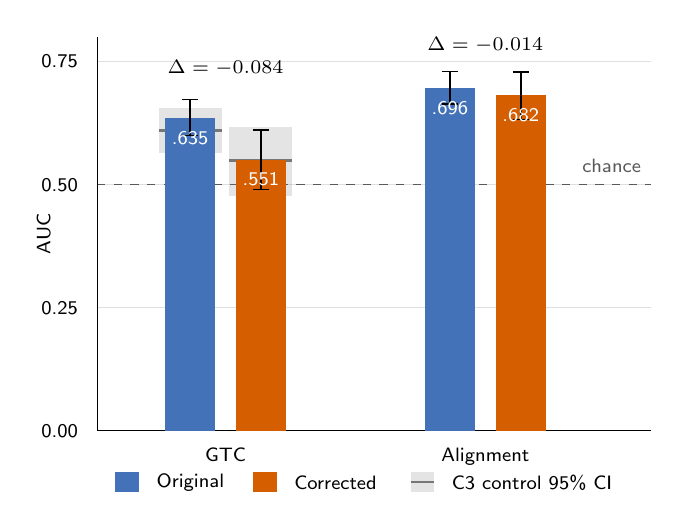
\begin{tikzpicture}[x=1cm,y=1cm,font=\sffamily\fontsize{7}{8}\selectfont]
  % Plot area: AUC 0--0.8 mapped to y=0--5.
  \foreach \value/\y in {0.00/0.000,0.25/1.563,0.50/3.125,0.75/4.688} {
    \draw[gray!25,line width=0.3pt] (0.72,\y) -- (7.75,\y);
    \node[anchor=east] at (0.60,\y) {\value};
  }
  \draw[black!65,dashed,line width=0.45pt] (0.72,3.125) -- (7.75,3.125);
  \node[anchor=south east,text=black!65] at (7.75,3.15) {chance};
  \draw[line width=0.45pt] (0.72,0) -- (7.75,0);
  \draw[line width=0.45pt] (0.72,0) -- (0.72,5.0);
  \node[rotate=90] at (0.04,2.5) {AUC};

  % C3 uniform-attention GTC 95% confidence intervals and point estimates.
  \fill[control,opacity=0.20] (1.50,3.531) rectangle (2.30,4.100);
  \draw[control,line width=0.8pt] (1.50,3.813) -- (2.30,3.813);
  \fill[control,opacity=0.20] (2.40,2.975) rectangle (3.20,3.863);
  \draw[control,line width=0.8pt] (2.40,3.431) -- (3.20,3.431);

  % Bars.
  \fill[original]  (1.58,0) rectangle (2.22,3.969);
  \fill[corrected] (2.48,0) rectangle (3.12,3.444);
  \fill[original]  (4.88,0) rectangle (5.52,4.350);
  \fill[corrected] (5.78,0) rectangle (6.42,4.263);

  % Bootstrap confidence intervals.
  \foreach \x/\lo/\hi in {1.90/3.750/4.206,2.80/3.063/3.819,5.20/4.150/4.563,6.10/3.950/4.556} {
    \draw[line width=0.55pt] (\x,\lo) -- (\x,\hi);
    \draw[line width=0.55pt] (\x-0.10,\lo) -- (\x+0.10,\lo);
    \draw[line width=0.55pt] (\x-0.10,\hi) -- (\x+0.10,\hi);
  }

  \node[anchor=north] at (2.35,-0.10) {GTC};
  \node[anchor=north] at (5.65,-0.10) {Alignment};
  \node[anchor=south] at (2.35,4.38) {$\Delta=-0.084$};
  \node[anchor=south] at (5.65,4.68) {$\Delta=-0.014$};
  \node[text=white] at (1.90,3.72) {.635};
  \node[text=white] at (2.80,3.20) {.551};
  \node[text=white] at (5.20,4.10) {.696};
  \node[text=white] at (6.10,4.01) {.682};

  % Legend.
  \fill[original] (0.95,-0.78) rectangle (1.25,-0.53);
  \node[anchor=west] at (1.35,-0.655) {Original};
  \fill[corrected] (2.70,-0.78) rectangle (3.00,-0.53);
  \node[anchor=west] at (3.10,-0.655) {Corrected};
  \fill[control,opacity=0.20] (4.70,-0.78) rectangle (5.00,-0.53);
  \draw[control,line width=0.8pt] (4.70,-0.655) -- (5.00,-0.655);
  \node[anchor=west] at (5.10,-0.655) {C3 control 95\% CI};
\end{tikzpicture}
\end{document}
